\documentclass[]{article}
\newcommand{\FileDepth}{../../..}
\usepackage[a4paper, total={15cm,23cm}]{geometry}
\usepackage[T1]{fontenc}
\usepackage{textcomp}%Not strictly necessary, but gives \textmu command for "micro."
\usepackage{fancyhdr}
\usepackage{amsmath}
\usepackage{amssymb}
\usepackage{graphicx}
\usepackage{xcolor}
\usepackage{tikz}
\usetikzlibrary{calc}
%opening
\newcommand{\SecType}{R}
\newcommand{\Week}{7}
\title{PH 221 Week \Week}
\author{Benjamin Bauml}
\date{Spring 2024}
\pagestyle{fancy}
\rhead{PH 221}
\chead{Spring 2024}
\lhead{Week \Week}

% For Assignment, leave Purpose as 1. For Worksheet, set to 2. For Student Solution, set to 3. For Teacher Solution, set to 4.
% If you want keep the pieces from being called manually, set DefOnly to 0.
\newcommand{\Purpose}{1}
\newcommand{\DefOnly}{1}

% Version 2024-04-27
% Changes
% 2024-02-21 Added xstring package to enable smooth implementation of new \ModePage command.
% 2024-04-27 Set up to split activities and formatting aspects into separate files. Removed dependence on xcomment. Added an automatic counter to number the activities in a problem set.
\usepackage{tcolorbox}
\usepackage{xstring}
% You will want the following four lines in your document (the last two uncommented):
% For Assignment, leave Purpose as 1. For Worksheet, set to 2. For Student Solution, set to 3. For Teacher Solution, set to 4.
% If you want keep the pieces from being called manually, set DefOnly to 0.
%\newcommand{\Purpose}{4}
%\newcommand{\DefOnly}{1}
\newcommand{\Exclusion}{0}
\newcommand{\PageTurn}{0}
\newcommand{\GrayProb}{0}
\newcommand{\Tipsy}{0}

% Assignment
\if\Purpose1
\renewcommand{\Exclusion}{1}
\fi
% Worksheet
\if\Purpose2
\renewcommand{\Exclusion}{1}
\renewcommand{\PageTurn}{1}
\fi
% Student Solution
\if\Purpose3
\renewcommand{\PageTurn}{1}
\renewcommand{\GrayProb}{1}
\fi
% Teaching Copy
\if\Purpose4
\renewcommand{\PageTurn}{1}
\renewcommand{\GrayProb}{1}
\renewcommand{\Tipsy}{1}
\fi

\def \NewQ {0}
\def \PForce {0}
\newcommand{\MaybePage}[1]{
	\def \PForce {#1}
	\if\PForce1
	\newpage
	\else
	\if\NewQ0
	\gdef \NewQ {\PageTurn}
	\else
	\newpage
	\fi
	\fi
}

\newcommand{\ModePage}[1]{
	\IfSubStr{#1}{\Purpose}{\newpage}{}
}

\newcounter{ActNumber}
\setcounter{ActNumber}{0}

\newcommand{\Problem}[4][0]{%The first argument is optional, and if it is set to 1, the \newpage will be forced. The second argument is the name of the activity, the third is the command the activity is stored as, and the fourth is the actual problem statement.
\newcommand{#3}{
\MaybePage{#1}
\addtocounter{ActNumber}{1}
\section*{\SecType\Week-\theActNumber: #2}
\if\GrayProb1
\begin{tcolorbox}[colback=lightgray,colframe=lightgray,sharp corners,boxsep=1pt,left=0pt,right=0pt,top=0pt,bottom=0pt,after skip=2pt]
\else
\begin{tcolorbox}[colback=white,colframe=white,sharp corners,boxsep=1pt,left=0pt,right=0pt,top=0pt,bottom=0pt,after skip=2pt]
\fi
#4
\end{tcolorbox}\noindent
}
\if\DefOnly0
\else
#3
\fi
}
	
\newcommand{\ProblemSub}[3][0]{%The first argument is optional, and if a string of numbers is entered into it, it will force a \newpage in any \Purpose that shows up in the string. For example, "13" would lead to the newpage being forced in modes 1 and 3. The second is the command the activity is stored as, and the third is the actual problem statement.
\newcommand{#2}{
\ModePage{#1}
\if\GrayProb1
\begin{tcolorbox}[colback=lightgray,colframe=lightgray,sharp corners,boxsep=1pt,left=0pt,right=0pt,top=0pt,bottom=0pt,after skip=2pt]
\else
\begin{tcolorbox}[colback=white,colframe=white,sharp corners,boxsep=1pt,left=0pt,right=0pt,top=0pt,bottom=0pt,after skip=2pt]
\fi
#3
\end{tcolorbox}\noindent
}
\if\DefOnly0
\else
#2
\fi
}
		
\newcommand{\Solution}[2]{%The first argument is the command the solution is stored as, and the second is the actual solution.
\newcommand{#1}{
\if\Exclusion0
#2
\fi
}
\if\DefOnly0
\else
#1
\fi
}
		
\newcommand{\ProblemFig}[2]{%The first argument is the command the figure is stored as, and the second is the actual figure.
\newcommand{#1}{
\begin{figure}[h]
#2
\end{figure}
}
\if\DefOnly0
\else
#1
\fi
}
		
\newcommand{\TeachingTips}[1]{
\if\Tipsy1
\begin{tcolorbox}[colback=lightgray,colframe=black]
#1
\end{tcolorbox}
\fi
}

%\newcommand{\FBDaxes}[3]{
	\begin{scope}[shift={(#1)},rotate=#2]
		% x-axis
		\draw[thick,->] (-2,0) -- (2,0);
		\node[anchor=west] at (2,0) {$x$};
		% y-axis
		\draw[thick,->] (0,-2) -- (0,2);
		\node[anchor=west] at (0,2) {$y$};
		\coordinate (#3) at (0,0);
	\end{scope}
}
\newcommand{\FBDvectorMA}[4]{
	\begin{scope}[shift={(#1)}]
		\coordinate (#4tip) at ({#2*cos(#3)},{#2*sin(#3)});
		\draw[ultra thick,blue,->] (#1) -- (#4tip);
	\end{scope}
}
\newcommand{\FBDvectorXY}[3]{
	\begin{scope}[shift={(#1)}]
		\coordinate (#3tip) at (#2);
		\draw[ultra thick,blue,->] (0,0) -- (#3tip);
	\end{scope}
}
\newcommand{\FBDdot}[1]{
	\filldraw[black] (#1) circle (3pt);
}% May want this to eventually replace the borrowed images.

\begin{document}
\maketitle
\begin{center}
	This material is borrowed/adapted from Chapter 9 of the \textit{Student Workbook} for \textit{Physics for Scientists and Engineers}.
\end{center}

\Problem{Visual Dot Product Practice}{\VisDotProdPracA}{
(a) If $ \vec{A}\cdot\vec{B} = 0 $, can you conclude that one of the vectors has zero magnitude? Explain.
}
\Solution{\VisDotProdPracASol}{No. The vectors $ \vec{A} $ and $ \vec{B} $ could be perpendicular to each other.}
\ProblemSub{\VisDotProdPracB}{
(b) For each pair of vectors, is the sign of $ \vec{A}\cdot\vec{B} $ positive (+), negative ($ - $), or zero (0)?
}
\ProblemFig{\VisDotProdPracBFig}{
\centering
\if\GrayProb1
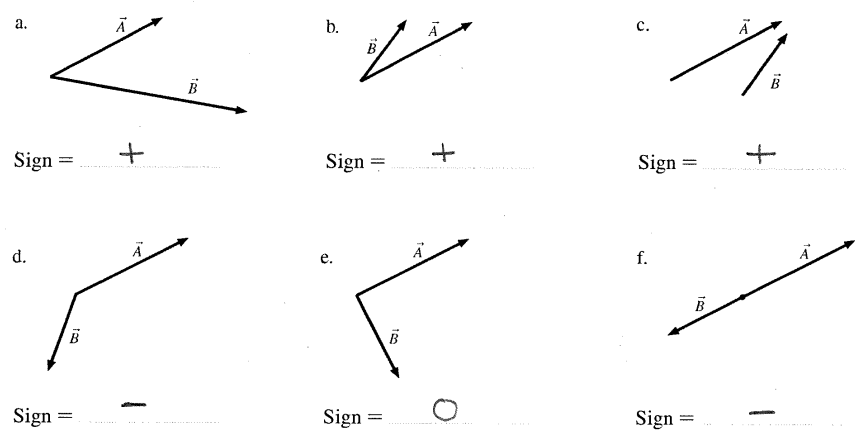
\includegraphics[scale=0.45]{\FileDepth/Activities/Visual_Dot_Product_Practice/Vectors_to_Dots_Solution.png}
\else
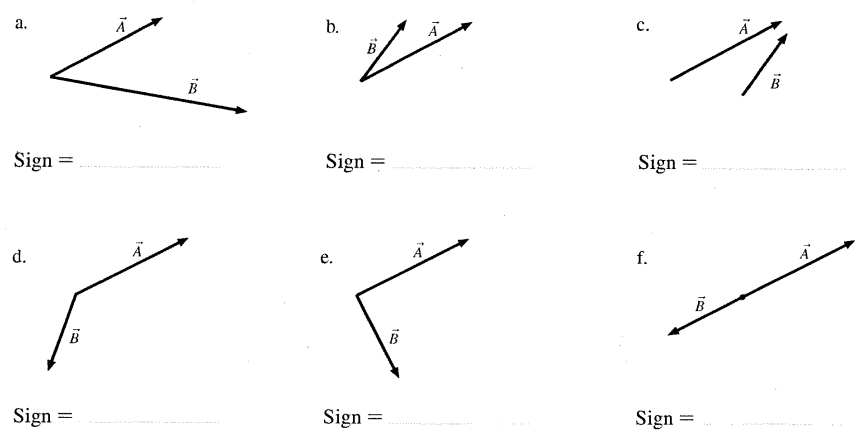
\includegraphics[scale=0.45]{\FileDepth/Activities/Visual_Dot_Product_Practice/Vectors_to_Dots_Blank.png}
\fi
}
\ProblemSub{\VisDotProdPracC}{
(c) Each of the diagrams below shows a vector $ \vec{A} $. Draw and label a vector $ \vec{B} $ that will cause $ \vec{A}\cdot\vec{B} $ to have the sign indicated.
}
\ProblemFig{\VisDotProdPracCFig}{
\centering
\if\GrayProb1
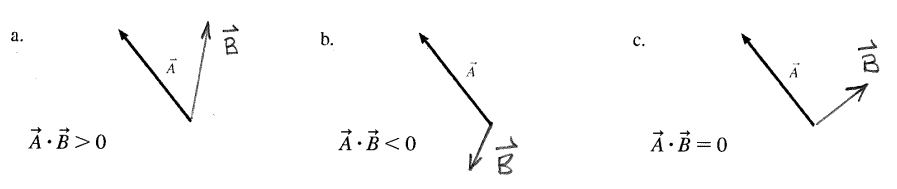
\includegraphics[scale=0.45]{\FileDepth/Activities/Visual_Dot_Product_Practice/Dots_to_Vectors_Solution.png}
\else
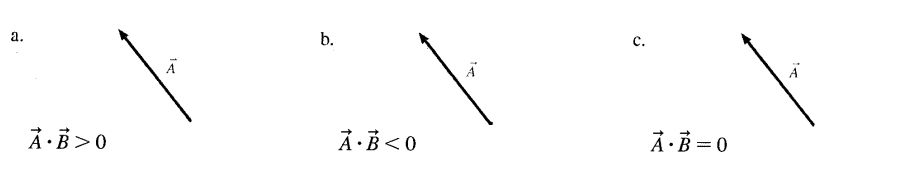
\includegraphics[scale=0.45]{\FileDepth/Activities/Visual_Dot_Product_Practice/Dots_to_Vectors_Blank.png}
\fi
}
\Problem{Lifting Boxes}{\LiftBox}{
Rudy picks up a 5 kg box and lifts it straight up, at constant speed, to a height of 1 m. Beth uses a rope to pull a 5 kg box up a 15$ ^{\circ} $ frictionless slope, at constant speed, until it has reached a height of 1 m. Which of the two does more work? Or do they do equal amounts of work? Explain.
}
\Solution{\LiftBoxSol}{

The amount of work done is the same for both. To raise an object higher, one must do work against gravity equal to $ mgh $ independent of the path taken to reach the height $ h $.

Using a work approach, we know that Rudy must be exerting a force of $ mg = (5 \text{ kg})(9.8\text{ m/s}^{2}) = 49 $ N up (opposing gravity) to lift the box at constant speed. The displacement is $ h = 1 $ m, and force and displacement are in the same direction, so the work done is $ W = mgh = 49 $ J. When Beth pulls the box up the $ \theta = 15^{\circ} $ slope, she must pull with $ mg\sin\theta $ to oppose the force of gravity parallel to the slope. We know that the height of the slope is $ h $, and if the length of the slope (the hypotenuse of the triangle it forms with the vertical axis and the ground) is $ L $, then we know that $ \sin\theta = \frac{h}{L} $, and thus the displacement of the box $ L = \frac{h}{\sin\theta} $. The force and displacement are in the same direction, so the work done by Beth is $ W = (mg\sin\theta)L = mgh = 49 $ J. Again, both do the same amount of work. Beth just does it over a longer distance with a lesser force.
}
\Problem{Spring Reasoning}{\SpringReas}{
A spring has an unstretched length of 10 cm. It exerts a restoring force $ F $ when stretched to a length of 11 cm.
}
\ProblemSub{\SpringReasA}{
(a) For what length of the spring is its restoring force $ 3F $?
}
\Solution{\SpringReasASol}{

Let us keep this very general for now. An ideal spring obeys Hooke's law:
\[
\vec{F}_{sp} = -k\Delta\vec{s},
\]
where $ k $ is the spring constant, and $ \Delta\vec{s} $ is the displacement of the end of the spring from its equilibrium position. Taking components along the $ s $-direction, we maintain the sign relationship between the force and the displacement, but remove the vector notation:
\[
F_{sp,s} = -k\Delta s.
\]
Let us have two situations: Case A, where we have some displacement $ \Delta s_{A} $ and a restoring force $ F_{sp,s,A} = -k\Delta s_{A} $, and Case B, where we have another displacement $ \Delta s_{B} $ and a restoring force $ F_{sp,s,B} = -k\Delta s_{B} $. Consider what happens when we divide one equation by the other:
\[
\begin{split}
	F_{sp,s,A} & = -k\Delta s_{A} \\
	\div(F_{sp,s,B} & = -k\Delta s_{B}) \\
	\implies \frac{F_{sp,s,A}}{F_{sp,s,B}} & = \frac{-k\Delta s_{A}}{-k\Delta s_{B}} = \frac{\Delta s_{A}}{\Delta s_{B}}.
\end{split}
\]
From this, we can see that if we triple the force from Case A to Case B, we must also triple the displacement. For our particular situation, we have a positive displacement $ \Delta s = 11\text{ cm} - 10\text{ cm} = 1 $ cm and therefore a negative restoring force $ -F $. If we desire triple the restoring force ($ -3F $), we get
\[
\frac{-F}{-3F} = \frac{1\text{ cm}}{\Delta s_{B}} \implies \Delta s_{B} = 3\text{ cm}.
\]
Thus, the spring's total length must be 13 cm.
}
\ProblemSub{\SpringReasB}{
(b) At what compressed length is the restoring force $ 2F $?
}
\Solution{\SpringReasBSol}{

For a compressed spring, the displacement is negative and the restoring force is positive. We have doubled the magnitude of the force, so the displacement must also be doubled in magnitude:
\[
\frac{-F}{2F} = \frac{1\text{ cm}}{\Delta s_{B}} \implies \Delta s_{B} = -2\text{ cm}.
\]
Thus, the spring must be 2 cm shorter than its equilibrium length, or 8 cm long.
}
\end{document}